\documentclass[a4paper,12pt]{article}

\usepackage[margin=2.5cm]{geometry}

\usepackage{polyglossia}
\usepackage{csquotes}

\usepackage[binary-units=true]{siunitx}
\usepackage[fleqn]{amsmath}

\usepackage{graphicx}
\usepackage{tabu}

\usepackage{hyperref}
\usepackage[bibencoding=utf8,backend=biber,sorting=none]{biblatex}

\setdefaultlanguage[spelling=new, babelshorthands=true]{german}

\hypersetup{
	pdfauthor={Leonard Hecker},
	pdftitle={Belegarbeit Internettechnologien 2},
	unicode=true,
}

\addbibresource{belegarbeit.bib}

\setlength{\parindent}{0pt}
\setlength{\parskip}{1em}

\begin{document}
\sloppy

\title{Belegarbeit Internettechnologien 2}
\date{\footnotesize \today}
\author{
	\small
	\begin{tabular}{rl}
		Vorname, Name: & Leonard Hecker \\
		Anschrift:     & August-Bebel-Str. 44, 01219 Dresden \\
	\end{tabular}
}

\setcounter{page}{0}
\maketitle
\thispagestyle{empty}

\clearpage
\section{Prolog}

Das vorliegende Projekt stellt eine nahezu vollständig konforme Implementierung der für die Aufgabenstellung wesentlichen Bestandteile von RTSP \cite{RFC2326}, RTP \cite{RFC3550}, sowie RTP-basierter FEC \cite{RFC5109} dar.

Das Projekt wurde innerhalb der Domain \texttt{hecker.io} in 3 Packages unterteilt:
\vspace{-1.5\topsep}
\begin{itemize}
	\setlength{\itemsep}{0em}
	\item \texttt{rtsp}: Eine generische RTSP Client/Server Implementierung
	\item \texttt{rtp}: Eine partiell generische RTP Sender/Receiver Implementierung, samt Unterstützung für MJPEG und FEC Pakete
	\item \texttt{it2}: Kombiniert die 2 überliegenden Packages um letztendlich die geforderten Fähigkeiten in Form einer CLI/GUI Anwendung zu implementieren
\end{itemize}

Es sei des Weiteren erwähnt, dass viele der enthaltenen Klassen von guava's \texttt{AbstractExecutionThreadService} erben.
Solcherlei Klassen erfüllen guava's \texttt{Service} Interface zum asynchronen Start, Stop sowie zur Überwachung des Servicezustands.
\texttt{AbstractExecutionThreadService} im besonderen führt hierbei zur Erfüllung des Interfaces die abstrakte Methode \texttt{run} in einem seperaten Worker-Thread aus.

\clearpage
\section{io.hecker.it2}

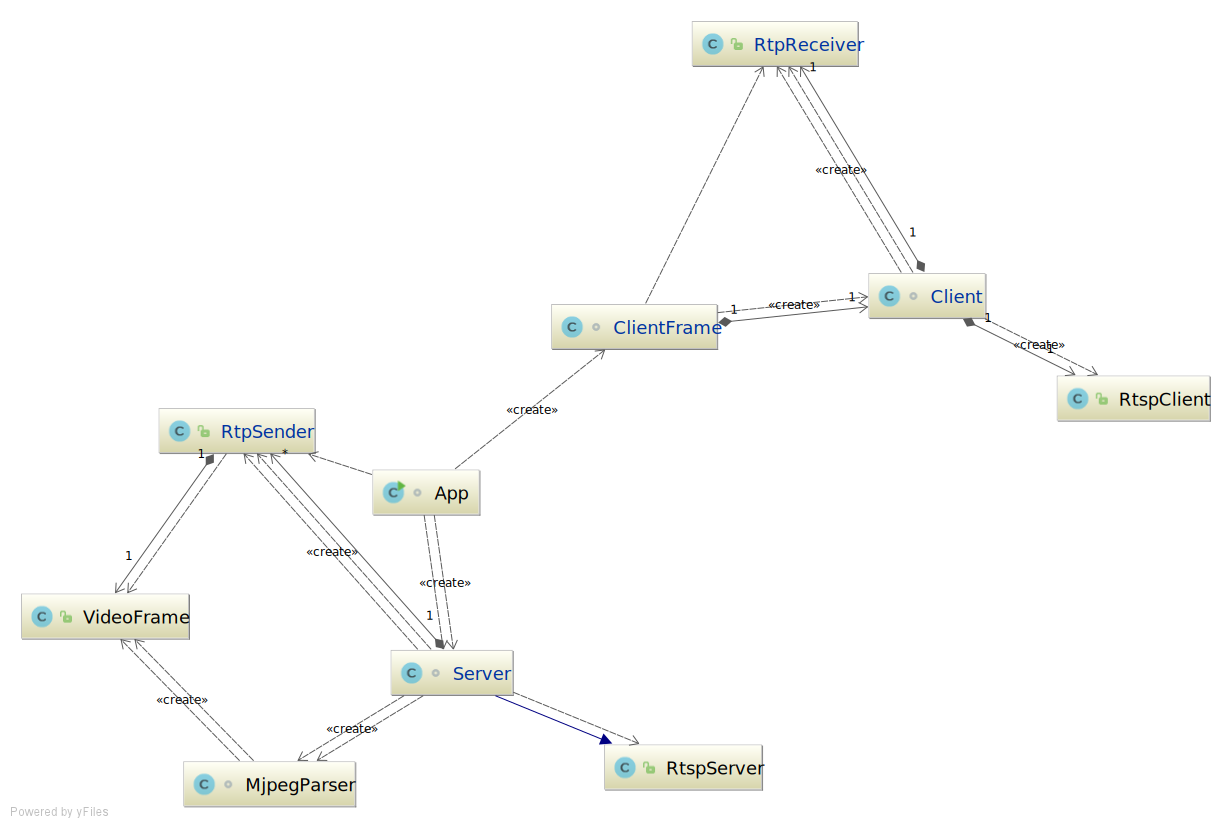
\includegraphics[width=\textwidth]{assets/it2.pdf}

An zentraler Stelle steht die Klasse \texttt{App}, welche die \texttt{main}-Funktion enthält.
Zunächst überträgt diese die \texttt{--loss} und \texttt{--fec} Parameterwerte an die \texttt{RtpSender} Klasse, damit diese später einen entsprechenden Paketverlust simuliert bzw. FEC-Korrektur anbietet.
Des Weiteren wird abhängig von dem \texttt{--server} Flag entweder eine \texttt{Server}, oder eine \texttt{ClientFrame} Instanz erzeugt, welche alle weiteren Tätigkeiten vornimmt.

\subsection{Server}

Die \texttt{Server} Klasse erbt von \texttt{RtspServer} und implementiert mithilfe dieser die geforderten, konkreten Methoden \texttt{OPTIONS}, \texttt{DESCRIBE}, \texttt{SETUP}, \texttt{TEARDOWN}, \texttt{PLAY} und \texttt{PAUSE}.

Wird ein \texttt{SETUP} Request erhalten, so wird mithilfe der Klasse \texttt{MjpegParser} die im Request-Pfad angegebene Datei - in diesem Fall \texttt{sample.mjpeg} - geöffnet und später in einzelne \texttt{VideoFrame}s geparsed.
Zeitgleich wird eine neue \texttt{RtpSender} Instanz erzeugt, welche später eben jene \texttt{VideoFrame}s konsumiert, jeweils in \texttt{RtpPacket}s umwandelt und diese als UDP Pakete zum angegebenen Empfänger sendet.
Bis zum Empfang eines \texttt{PLAY} Requests ist jedoch der \texttt{RtpSender} zunächst in einem pausierten Zustand.
Der \texttt{Client} erhält nun vom \texttt{Server} eine Session ID, welche für weitere Requests verwendet werden kann.

Erhält der \texttt{Server} einen Request, so wird dieser mithilfe der übergebenen Session ID den entsprechenden \texttt{RtspSender} suchen und diesen zerstören.

\texttt{TEARDOWN}, \texttt{PLAY} und \texttt{PAUSE} Requests hingegen sind relativ simpel implementiert und suchen jeweils nur den zur, im Request angegebenen, Session ID entsprechenden \texttt{RtspSender} und zerstören, de-pausieren bzw. pausieren ihn.

\subsection{ClientFrame}

Die \texttt{ClientFrame} Klasse erbt von \texttt{JFrame} um eine GUI Anwendung zu erzeugen.
Sie nutzt primär die namensgebende \texttt{Client} Klasse um jegliches RTSP, sowie RTP Handling zu vollführen und leitet alle UI-Interaktionen stellvertretend an diese weiter.

\subsection{Client}
Die \texttt{Client} Klasse erzeugt während des Startups einen \texttt{RtpReceiver} und sendet einen \texttt{SETUP} Request an den angegeben Server.
Analog wird während des Shutdowns ein \texttt{TEARDOWN} Request durchgeführt.
Die hierdurch beim Setup vom Server erhaltene Session ID wird nun für alle weiteren Abläufe verwendet.
Klickt der Nutzer auf das Video-Canvas im \texttt{ClientFrame}, wird, abhängig davon ob das Video aktuell pausiert ist oder nicht, ein entsprechender \texttt{PLAY} bzw. \texttt{PAUSE} Request gesendet.

\clearpage
\section{io.hecker.rtsp}

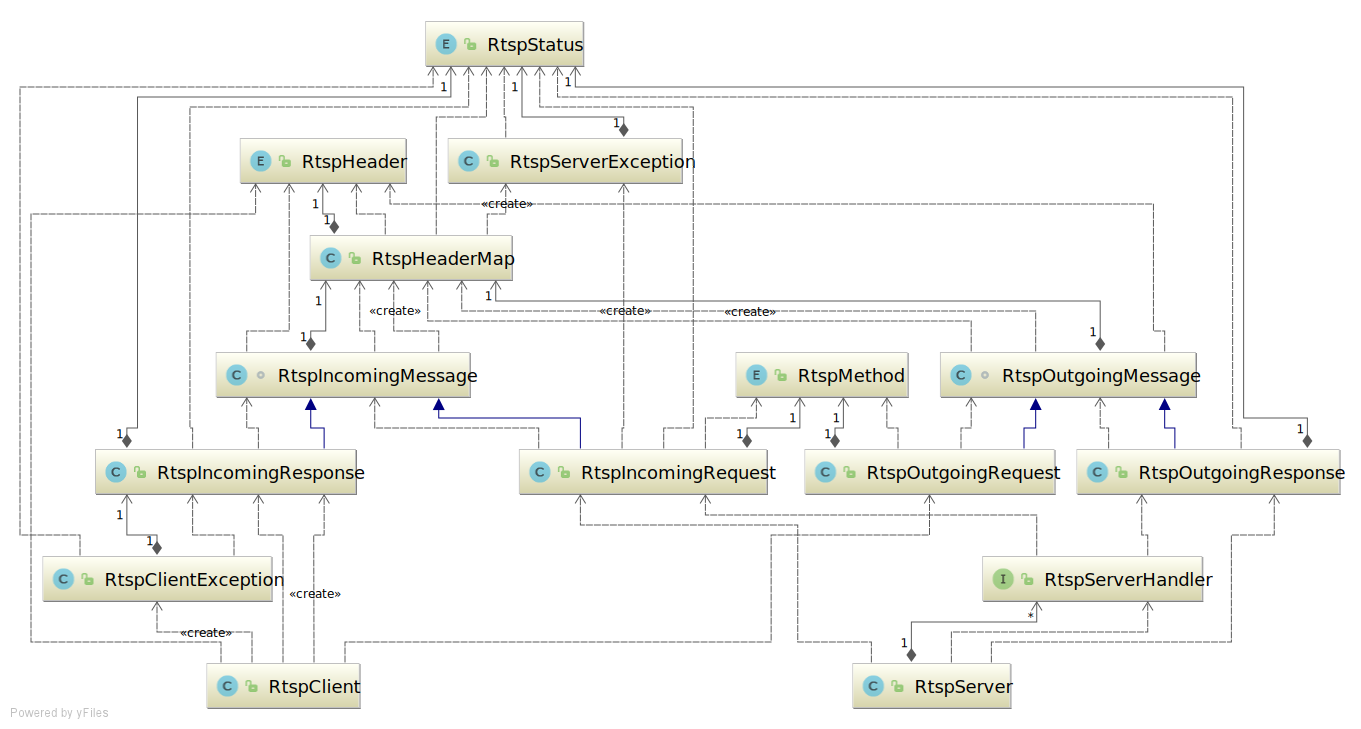
\includegraphics[width=\textwidth]{assets/rtsp.pdf}

In der RTSP \cite{RFC2326} Implementierung stehen an zentraler Stelle die Klassen \texttt{RtspClient} sowie \texttt{RtspServer}.

\subsection{RtspClient}

\texttt{RtspClient} implementiert einen generischen RTSP Client.
Zur Durchführung eines Request mittels der \texttt{fetch} Methode wird eine Instanz der Klasse \texttt{RtspOutgoingRequest} übergeben.
Nach der internen, automatischen Generierung des \texttt{CSEQ} Headers wird dann der Request serialisiert und gesendet.
Daraufhin wird eine \texttt{RtspIncomingResponse} erzeugt und mithilfe dieser die Response des Servers eingelesen, deserialisiert und zurückgegeben.

\subsection{RtspServer}

\texttt{RtspServer} implementiert einen generischen RTSP Server.
Bei diesem können mittels der \texttt{addHandler} Methode eine beliebige Anzahl an \texttt{RtspServerHandler} Callbacks registriert werden, welche dann für jeden Request aufgerufen werden, diesen inspizieren und Response-Daten setzen können.

Wurde eine TCP Connection angenommen, wird nun für jede einzelne ein \texttt{RtspServer.Connection} Service gespawnt.
Dieser erzeugt daraufhin in einer Dauerschleife \texttt{RtspIncomingRequest} Instanzen und liest und deserialisiert mit diesen einzelne Requests.
Zusammen mit einer noch leeren \texttt{RtspOutgoingResponse} Instanz wird so bei jedem Request nun die Liste aller registrierten \texttt{RtspServerHandler} aufgerufen.
Die vorliegende Server-Implementierung fügt hierbei automatisch bereits einige Standard-Header hinzu, wie z.B. den strikt verlangten \texttt{Date} Header, sowie \texttt{CSEQ} und \texttt{Content-Type}.
Die \texttt{RtspOutgoingResponse} Instanz wird letztendlich serialisiert und an den Client gesendet.

\subsection{RtspServerHandler}

Das \texttt{RtspServerHandler} Interface wird vom Server genutzt um bei diesem Callbacks bzw. Handler zu registrieren.
Jeder \texttt{RtspServerHandler} wird dann vom Server mit den aktuellen Request/Response-Paar aufgerufen und erlaubt dem Anwender den Request zu inspizieren und die Response beliebig mit Daten zu füllen.

Es ist hierbei möglich eine \texttt{RtspServerException} zu werfen.
Diese wird vom \texttt{RtspServer} aufgefangen und der darin enthaltene Status Code in der Response gesetzt.

\subsection{RtspIncoming*}

\texttt{RtspIncomingRequest} sowie \texttt{RtspIncomingResponse} erben von \texttt{RtspIncomingMessage}, welches die Deserialisierung der Headerzeilen mittels einer \texttt{RtspHeaderMap} sowie die des Bodys implementiert.
\texttt{RtspIncomingRequest} und \texttt{RtspIncomingResponse} fügen hierbei nur noch das Einlesen der jeweiligen Statuszeile hinzu um die Funktionalität zu vervollständigen.

\subsection{RtspOutgoing*}

\texttt{RtspOutgoingRequest} sowie \texttt{RtspOutgoingResponse} erben von \texttt{RtspOutgoingMessage}, welches die Serialisierung der Headerzeilen mittels der enthaltenen \texttt{RtspHeaderMap} sowie die des Bodys implementiert.
\texttt{RtspOutgoingRequest} und \texttt{RtspOutgoingResponse} fügen hierbei nur noch das Erzeugen der jeweiligen Statuszeile hinzu um die Funktionalität zu vervollständigen.

\subsection{RtspHeaderMap}

\texttt{RtspHeaderMap} stellt ein vereinfachtes \texttt{Map} Interface für Request/Response Header dar.
Des Weiteren wird hier die Deserialisierung sowie Serialisierung der Headerzeilen von einem \texttt{DataInput} sowie in ein \texttt{DataOutput} implementiert.

\subsection{RtspStatus}

Das Enum \texttt{RtspStatus} enthält alle unterstützten RTSP Statuscodes.

\subsection{RtspMethod}

Das Enum \texttt{RtspMethod} enthält alle unterstützten RTSP Anfragemethoden.

\clearpage
\section{io.hecker.rtp}

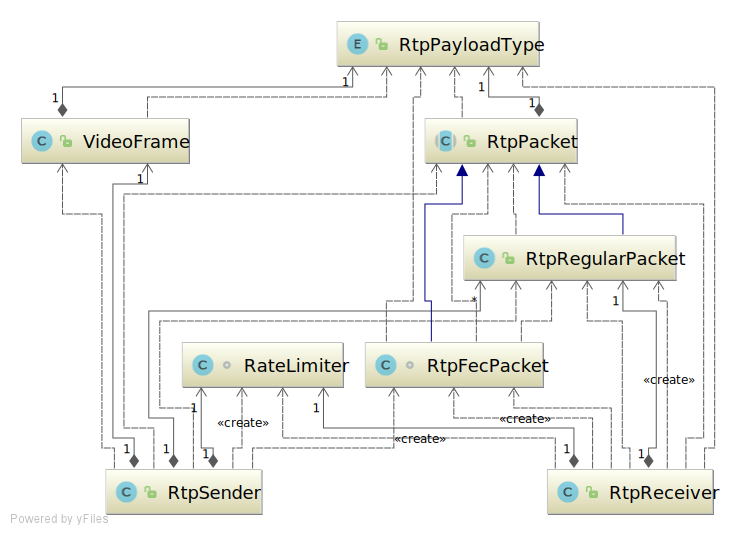
\includegraphics[width=\textwidth]{assets/rtp.pdf}

In der RTP \cite{RFC3550} Implementierung stehen an zentraler Stelle die Klassen \texttt{RtpSender} sowie \texttt{RtpReceiver}.

\subsection{RtpSender}

Die \texttt{RtpSender} Klasse wird mit einer Zieladresse und einem \texttt{VideoFrame} Iterator konstruiert, wandelt letzteres in eine Serie von \texttt{RtpPacket} Instanzen um und sendet diese an die angegebene Zieladresse.

Die Implementierung des \texttt{RtpSender} ist weitestgehend sehr simpel.
Mittels einem \texttt{RateLimiter} wird die Rate des Einlesens vom \texttt{VideoFrame} Iterator und des Sendens derart gesteuert, dass dies der Framerate des Videos entspricht.
Wurde ein \texttt{RtpRegularPacket} gesendet, so wird dieses nur noch optional der FEC Queue hinzugefügt.

Sofern das \texttt{--fec} Flag gesetzt und der äquivalente \texttt{FEC\_SIZE} Wert größer $0$ ist, wird nun das Paket der \texttt{m\_fecQueue} hinzugefügt.
Enthält die \texttt{m\_fecQueue} mindestens \texttt{FEC\_SIZE} Elemente, so werden die darin enthaltenen Pakete zu einem einzelnen \texttt{RtpFecPacket} kodiert und dem Empfänger gesendet.

\subsection{RtpReceiver}

Die \texttt{RtpReceiver} Klasse ist ein \texttt{Service}, welcher asynchron im Hintergrund UDP Pakete empfängt und diese mittels der \texttt{RtpPacket} Klasse etc. deserialisiert.

Primär empfängt ein \texttt{RtpReceiver} Pakete des Typs \texttt{RtpRegularPacket}.
Diese werden hierbei in der Queue \texttt{m\_queue} für eine spätere entnahme abgelegt.
Die Queue ist hierbei eine \texttt{PriorityQueue} welche anhand der Sequence Number bzw. alternativ anhand des Timestamp der enthaltenen Pakete sortiert wird.
Auf diese Weise werden später Out-of-Order Pakete trotz dessen in der richtigen Reihenfolge entnommen.

Wird ein \texttt{RtpFecPacket} empfangen, wird diesem die aktuelle Queue übergeben, mithilfe welcher die \texttt{RtpFecPacket} Implementierung bis zu ein verloren gegangenes Paket widerherstellen kann.

Im gegenüberliegenden Fordergrund steht die Methode \texttt{next} mit welcher Pakete aus der Queue entnommen werden können.
Hierbei steht der Monitor \texttt{m\_queueMonitor} an zentraler Stelle zur Synchronisation mit dem im Hintergrund laufenden Service.

Enthält die Queue weniger als $16$ Pakete, z.B. weil der Stream noch nicht gestartet hat, so wird zunächst gewartet bis dies der Fall ist.
Die hierbei verwendete Logik erlaubt es zusätzlich bis zu $\SI{3}{\second}$ zu warten bis die Queue optional bis zu $32$ Pakete enthält.
Dies stellt einerseits sicher, dass immer alle bis zu $16$ Pakete, welche von einem \texttt{RtpFecPacket} referenziert werden können, in der Queue auffindbar sind und andererseits, dass beim Start des Streams ein möglichst großer Buffer vorhanden ist um etwaige Latenzschwankungen etc. auszugleichen.

Enthält die Queue nun genügend Pakete, so wird äquivalent zum \texttt{RtpSender} mittels einem \texttt{RateLimiter} und dem Monitor gewartet bis das nächste RTP Paket angezeigt werden kann.
Ändert sich aufgrund von Out-of-Order Paketen oder FEC Reperatur die Spitze der Queue und somit das voraussichtlich als nächstes anzuzeigende Paket, so ändert sich demzufolge auch die Wartezeit.
Dies wird mittels dem \texttt{QueueHeadChangedGuard} und dem Monitor überwacht und in einem solchen Falle der Warteprozess mit dem Timestamp des neuen Queue Head von neuem gestartet.

\subsection{RtpPacket}

Die abstrakte Klasse \texttt{RtpPacket} implementiert die gemeinsame Funktionalität der Klassen \texttt{RtpRegularPacket} und \texttt{RtpFecPacket}: Die Serialisierung, Deserialisierung und einen Builder für alle statischen Felder eines RTP Packets, definiert in RFC3550 \cite{RFC3550}, Sektion 5.1.
Der optionale Extension Header, sowie das Auslesen von \texttt{CSRC} Feldern wurde hierbei jedoch nicht implementiert.

Diese Klasse und ihre beiden Implementierungen machen sich des Weiteren das Builder-Pattern zu nutze, um elegant immutable Instanzen zu erzeugen.

\subsection{RtpRegularPacket}

\texttt{RtpRegularPacket} ist eine schlanke Erweiterung des \texttt{RtpPacket} und fügt einzig das Serialisieren und Deserialisieren des Payloads hinzu.

\subsection{RtpFecPacket}

\texttt{RtpFecPacket} implementiert RTP-basierte FEC.
Während die Implementierung der Serialisierung und Deserialisierung von Paketen vollständig RFC5109 \cite{RFC5109},  Sektion 7, folgt, bietet die triviale Implementierung der Recovery jedoch nur Unterstützung von FEC Level 0.

\subsection{RateLimiter}

Die Klasse \texttt{RateLimiter} dient dem \texttt{RtpSender} sowie dem \texttt{RtpReceiver} dazu, die Rate des Sendens bzw. Anzeigens zu steuern.
Die Klasse implementiert im Kern den folgenden Algorithmus:
\begin{align*}
P_{n+1} &= P_n + \left( T_{n+1} - T_n \right) \\
S &= P_{n+1} - Z_n
\end{align*}

Mit:
\vspace{-1.5\topsep}
\begin{itemize}
	\setlength{\itemsep}{0em}
	\item $P$: Zeitstempel der letzten Präsentation
	\item $T$: Paketzeitstempel
	\item $Z$: Aktuelle Zeit
	\item $S$: Dauer die geschlafen werden muss um das Rate Limit zu erfüllen
\end{itemize}

Dies stellt sicher, dass kleinere temporale Fluktuenzen zwischen den Aufrufen der Methoden des \texttt{RateLimiter} herausgefiltert werden und somit, dass über die Dauer des Streamings hinweg kein Zeitdrift auftritt.

\clearpage
\section{Epilog}

Ein zufriedenstellender Wert für $k$ wurde auf theoretische Weise ermittelt.
Die \texttt{sample.mjpeg} Datei ist $\SI{4269893}{\byte}$ groß und enthält $500$ Frames mit jeweils einem $\SI{5}{\byte}$ Header.
Dies entspricht einer durchschnittlichen Payloadgröße von $\SI{8535}{\byte}$, sowie der kumulativen Gesamtgröße aller Frames von $\SI{4267393}{\byte}$.
Aufgrund der signifikanten Größe des durchschnittlichen Payloads wird im folgenden die Größe des RTP und FEC Headers in Berechnungen vernachlässigt.

Des Weiteren werden die Konstanten
\begin{align*}
p &= 0.1 \\
G &= \SI{4267393}{\byte}
\end{align*}
angenommen.

\begin{tabu} to \linewidth { l | X | X | X | X | X }
	$k$  & Qualität & Datenmenge & $Q_q$  & $Q_d$  & Score \\ \hline
	$2$  & $0.99$   & $5760981$  & $1.00$ & $0.00$ & \\
	$3$  & $0.97$   & $5120872$  & $0.96$ & $0.38$ & $0.37$ \\
	$4$  & $0.95$   & $4800817$  & $0.91$ & $0.57$ & $0.52$ \\
	$5$  & $0.92$   & $4608784$  & $0.85$ & $0.69$ & $0.58$ \\
	$6$  & $0.89$   & $4480763$  & $0.78$ & $0.76$ & $0.59$ \\
	$7$  & $0.85$   & $4389319$  & $0.71$ & $0.82$ & $0.58$ \\
	$8$  & $0.81$   & $4320735$  & $0.63$ & $0.86$ & $0.54$ \\
	$9$  & $0.77$   & $4267393$  & $0.55$ & $0.89$ & $0.49$ \\
	$10$ & $0.74$   & $4224719$  & $0.47$ & $0.91$ & $0.43$ \\
	$11$ & $0.70$   & $4189804$  & $0.38$ & $0.94$ & $0.36$ \\
	$12$ & $0.66$   & $4160708$  & $0.30$ & $0.95$ & $0.29$ \\
	$13$ & $0.62$   & $4136089$  & $0.22$ & $0.97$ & $0.22$ \\
	$14$ & $0.58$   & $4114986$  & $0.15$ & $0.98$ & $0.14$ \\
	$15$ & $0.55$   & $4096697$  & $0.07$ & $0.99$ & $0.07$ \\
	$16$ & $0.51$   & $4080695$  & $0.00$ & $1.00$ & \\
\end{tabu}

Die \textit{Qualität} entspricht hierbei der Wahrscheinlichkeit, dass ein Paket verloren geht.
Dies wurde mithilfe von Bernoulli's unteren, kumulativen Verteilungsfunktion ${F(k,n,p) = P(X \leq k)}$ berechnet.
Hierbei entsprechen, gemäß der üblichen Benennung der Parameter der Verteilungsfunktion, der Parameter $k$ der Anzahl an Erfolgen, welcher im Falle einer gerade noch gelingenden Level 0 FEC Recovery $1$ beträgt, der Parameter $n$ den in der Aufgabenstellung und in der obigen Tabelle verwendeten Parameter $k$, sowie $p$ der konstanten Verlustrate $0.1$.

Die \textit{Datenmenge} $D$ berechnet sich des Weiteren mittels:
\begin{align*}
D &= \left(G + \frac{G}{k}\right) * \left(1 - p \right)
\end{align*}
Hierbei wurde die Berechnung des Overheads der FEC Pakete vereinfacht und mit dem Näherungswert $G \div k$ ausgedrückt.

Die Spalten $Q_{q/d}$ sollen hierbei auf einfache Weise die Qualitätsmerkmale quantifizieren.
Hierbei wird $Q_q$, dem Quantum der Qualität, sowie $Q_d$, dem Quantum der Datenmenge, die Werte $1$ für das Beste und $0$ für das Schlechteste jeweilige Ergebnis zugeordnet.
Alle zwischenliegende Werte erhielten ein linear interpolierten Wert.

Der endgültige \textit{Score} entspricht dem Produkt $Q_q * Q_d$.

\textit{Hierbei stellt sich $k = 6$ als ein gute Balance zwischen Datenmenge und Qualität heraus.}

\clearpage
\printbibliography

\end{document}
